% !TEX TS-program = xelatex
% !BIB program = biber
% !TEX encoding = UTF-8 Unicode

% 使用手冊請見 TW_Thesis_Template wiki:
% https://github.com/sppmg/TW_Thesis_Template/wiki

% User guide in wiki of TW_Thesis_Template :
% https://github.com/sppmg/TW_Thesis_Template/wiki

\documentclass[openany]{NTHU_thesis} % \documentclass[option1, option2, ...]
% Helpful options: 
% draft = Don't load figure ,reduce compile time.
% showframe = show document margins.
% colorgrid = show colored coordinate. (by eso-pic pkg.)
% openany: see issue #5, NTHU not allow blank page, so add this option to allow chapter start in left side,
\usepackage[subpreambles]{standalone} % standalone class setting in config.tex
% Option ``subpreambles'' enable sub-tex's preambles when compile main tex. (pkg default disable)
% sppmg think it's still some problem (e.g. \addbibresource will faild ), recommend move all subpreambles to ``macros_preamble.tex``

\begin{document}
    \frontmatter
        \documentclass[class=NTU_thesis, crop=false, float=true]{standalone}

\begin{document} 
\def\fsUniversityZh{\fontsize{18}{27}\selectfont }
\def\fsUniversityEn{\fontsize{16}{24}\selectfont }
\def\fsDeptEn{\fontsize{14}{21}\selectfont }
\def\fsTitle{\fontsize{18}{27}\selectfont }
\def\fsNames{\fs{18}[1.5] }
% --------define title page layout for thesis
\rmfamily
\ifthenelse{\boolean{disableChinese}}{}{
    \CJKfamily{sf} % use roman font for en, kai(sf) for zh
}
\newgeometry{top=4cm, bottom=3cm, inner=2cm, outer=2cm} % only for titlepage
\begin{spacing}{1.0}
\begin{titlepage}
%     \null\vfill
    \begin{center}
        {\fsUniversityZh\textbf{國立台灣大學~\deptZh} \par
            \textbf{\degreeZh 論文} \par}
        \vspace*{5mm}
        {\fsDeptEn \deptEn \par}
        {\fsUniversityEn 
            National Taiwan University \par
            \degreeEn\ Thesis\par}
        \vspace*{10mm}
        
        {\fsTitle {\titleZh} \par}
        \vspace*{5mm}
        {\fsTitle {\titleEn} \par}
        \vspace*{10mm}
        
        {\ifx \logo\empty\vfill
        \else 
\includegraphics[height=30mm]{\logo}\vfill\vspace*{3mm} \par
        \fi}
        {\fsNames
        \authorZh \par
        \authorEn \par}
        \vspace*{10mm}
        
        {\fsNames \renewcommand{\arraystretch}{1}
        \begin{tabular}{ll@{\quad}r}
        指導教授: & \mprofZh  & 博士   \\
        \ifx \sprofiZh\empty \else
                 & \sprofiZh  & 博士  \\ \fi
        \ifx \sprofiiZh\empty \else
                 & \sprofiiZh & 博士  \\ \fi
        \end{tabular}\par}
        \vspace*{5mm}
        
        {\fsNames \renewcommand{\arraystretch}{1}
        \begin{tabular}{ll}
        Advisor: & \mprofEn   , Ph.D \\
        \ifx \sprofiEn\empty \else
                 & \sprofiEn  , Ph.D \\ \fi
        \ifx \sprofiiEn\empty \else
                 & \sprofiiEn , Ph.D \\ \fi
        \end{tabular}\par}
        \vspace*{5ex}
        
        \vfill
        
        {\fsTitle \degreedateROC \par
            \degreedateEn \par}
        
        \ifthenelse{\boolean{printcopyright}}
        {\vspace*{2ex}
        版權所有\copyright\ \author\ \copyyear \par}
    \end{center}
\end{titlepage}
\end{spacing}
\restoregeometry
\rmfamily % use main font
%--------end of title page for thesis
\cleardoublepage

\end{document}
       % 封面(不加浮水印)
        \documentclass[class=NTU_thesis, crop=false, float=true]{standalone}

\begin{document} 
\def\fsUniversityZh{\fontsize{18}{27}\selectfont }
\def\fsUniversityEn{\fontsize{16}{24}\selectfont }
\def\fsDeptEn{\fontsize{14}{21}\selectfont }
\def\fsTitle{\fontsize{18}{27}\selectfont }
\def\fsNames{\fs{18}[1.5] }
% --------define title page layout for thesis
\rmfamily
\ifthenelse{\boolean{disableChinese}}{}{
    \CJKfamily{sf} % use roman font for en, kai(sf) for zh
}
\newgeometry{top=4cm, bottom=3cm, inner=2cm, outer=2cm} % only for titlepage
\begin{spacing}{1.0}
\begin{titlepage}
%     \null\vfill
    \begin{center}
        {\fsUniversityZh\textbf{國立台灣大學~\deptZh} \par
            \textbf{\degreeZh 論文} \par}
        \vspace*{5mm}
        {\fsDeptEn \deptEn \par}
        {\fsUniversityEn 
            National Taiwan University \par
            \degreeEn\ Thesis\par}
        \vspace*{10mm}
        
        {\fsTitle {\titleZh} \par}
        \vspace*{5mm}
        {\fsTitle {\titleEn} \par}
        \vspace*{10mm}
        
        {\ifx \logo\empty\vfill
        \else 
\includegraphics[height=30mm]{\logo}\vfill\vspace*{3mm} \par
        \fi}
        {\fsNames
        \authorZh \par
        \authorEn \par}
        \vspace*{10mm}
        
        {\fsNames \renewcommand{\arraystretch}{1}
        \begin{tabular}{ll@{\quad}r}
        指導教授: & \mprofZh  & 博士   \\
        \ifx \sprofiZh\empty \else
                 & \sprofiZh  & 博士  \\ \fi
        \ifx \sprofiiZh\empty \else
                 & \sprofiiZh & 博士  \\ \fi
        \end{tabular}\par}
        \vspace*{5mm}
        
        {\fsNames \renewcommand{\arraystretch}{1}
        \begin{tabular}{ll}
        Advisor: & \mprofEn   , Ph.D \\
        \ifx \sprofiEn\empty \else
                 & \sprofiEn  , Ph.D \\ \fi
        \ifx \sprofiiEn\empty \else
                 & \sprofiiEn , Ph.D \\ \fi
        \end{tabular}\par}
        \vspace*{5ex}
        
        \vfill
        
        {\fsTitle \degreedateROC \par
            \degreedateEn \par}
        
        \ifthenelse{\boolean{printcopyright}}
        {\vspace*{2ex}
        版權所有\copyright\ \author\ \copyyear \par}
    \end{center}
\end{titlepage}
\end{spacing}
\restoregeometry
\rmfamily % use main font
%--------end of title page for thesis
\cleardoublepage

\end{document}
       % 書名頁
        \listoftodos   % todo list, hide when set \textbackslash{}setboolean\{publish\}\{\textbf{true}\} in config.tex. It will not add to TOC , you can add \todototoc before \listoftodos to do that.
            \todo[inline]{``Todo List'' will hide when set \textbackslash{}setboolean\{publish\}\{\emph{true}\} in config.tex.}

        %%%%%%%%%%%% letters %%%%%%%%%%%%
        % Set file name in config.tex
        % 依校方規定,此處須插入:
        % [v] 清大(電子授權書) 必備,不論是否授權都要裝訂
        % [v] 清大(紙本授權書) 必備,不論是否授權都要裝訂
        % [x] 國家圖書館(電子授權書) 有授權才要裝訂
        % [v] 國家圖書館(紙本論文延後公開/下架申請書)→紙本論文有申請延後公開才要裝訂
        % [v] 指導教授推薦書
        % [v] 考試委員審定書
        % !!! [x] 部份請自行插入

        % 碩博士論文電子檔授權書 Authorization Letter (for electronic)
        \IfFileExists{\letterAuthEl}{
            \cleardoublepage        % 由下個右頁開始
            \includepdf{\letterAuthEl}}{}
        % 碩博士論文紙本授權書 Authorization Letter (for paper)
        \IfFileExists{\letterAuthPa}{
            \cleardoublepage        % 由下個右頁開始
            \includepdf{\letterAuthPa}}{}
        % 國家圖書館(電子授權書) 有授權才要裝訂

        % 碩博士紙本論文延後公開/下架申請書。(如需延後公開者,才需要裝訂於論文內頁)
        \IfFileExists{\letterPubReq}{
            \cleardoublepage
            \includepdf{\letterPubReq}}{}
        % 指導教授推薦書
        \IfFileExists{\letterRecom}{
            \cleardoublepage
            \includepdf{\letterRecom}}{}
        % 口試委員審定書
        \IfFileExists{\letterVerif}{
            \cleardoublepage
            \includepdf{\letterVerif}}{}
        \cleardoublepage
        
        %%%%%%%%%%%% Other frontmatter, eg,abstract %%%%%%%%%%%%
        % 中英文論文摘要:內容應說明研究目的,資料來源,研究方法及研究結果等
        \documentclass[class=NCU_thesis, crop=false]{standalone}
\begin{document}

\chapter{摘要}
在此寫上你的中文摘要。

\vspace{2em}
\noindent \textbf{關鍵字:} \keywordsZh{} % Set keywords in config.tex
\end{document} % zh 中文摘要
        \documentclass[class=NCU_thesis, crop=false, float=true]{standalone}
\begin{document}
% This file is common document region, 
% it will loading when LaTeX see ``\begin{document}'' 
% It's for some command which need use in document region.
% DON'T put preamble only command in here, eg. \usepackage
% --------------------------------------------------

% standalone setting for sub-tex. (not every class option can use \standaloneconfig)
\IfStandalone{\standaloneconfig{float=true}}{} 
% ``float=false'' disable floating environment when build sub-tex.

% Old method for change font size, but no limit for size so keep here.
% \fontsize{size}{baselineskip} 無級調大小、行高, 行高倍數 = baselineskip/size/1.2 ,詳見教學。
% \fontsize{14}{25}\selectfont  

\ifzh{
    \setlength{\parindent}{2em} % 中文段首縮排2中文字寬
}{}                             % 英文照 LaTeX 預設


\chapter{Abstract}
Write your English abstract here.



\vspace{2em}
\noindent \textbf{Keywords:} \keywordsEn{} % Set keywords in config.tex
\end{document} % en 英文摘要
        \documentclass[class=NCU_thesis, crop=false]{standalone}
\begin{document}

\chapter{誌謝}

感謝中央大學、中央研究院提供的資源。Donald Ervin Knuth 的 \TeX\ ,Linus與眾多自由軟體好手提供的GNU/Linux。
另外特別感謝sppmg提供的論文樣板與教學\cite{_sppmg/tw_thesis_template_????},
讓我將學習\LaTeX\ 的時間拿來充實論文內容。(以上為sppmg自肥 XD)

\begin{figure}[!hbt]
    \captionsetup[subfigure]{labelformat=empty}
    \centering
    \subcaptionbox
        {}
        {
\includegraphics[width=0.2\linewidth]{logo-NCU.jpg}}
    ~
    \subcaptionbox
        {}
        {
\includegraphics[width=0.2\linewidth]{logo-sinica.png}}
    ~
    \subcaptionbox
        {}
        {
\includegraphics[width=0.2\linewidth]{logo-GNU.png}}
    ~
    \subcaptionbox
        {}
        {
\includegraphics[width=0.2\linewidth]{logo-Linux.png}}
    % \vspace{\baselineskip} % 分隔上下列	
\end{figure}


\end{document}


 % 誌謝(可略)

        % 原始 book class 不將 TOC,LOF,LOT 加入目錄列表,須手動加
        % 此樣板可由 config.tex 切換是否自動加入目錄
        \tableofcontents        % 目錄
        \listoffigures          % 圖目錄
        \listoftables           % 表目錄
        \documentclass[class=NCU_thesis, crop=false]{standalone}
\begin{document}

\chapter{Symbol}
Use table for symbol list

\begin{table}[h]
	\fontsize{14}{25}\selectfont  % 使用與內文一樣大的字體,請自調
	\centering
	\begin{tabular}{c@{\quad}@{:}l}
% 		符號		& \ 說明 \\ 
		VIM     & The best guy's editor \\ 
		Emacs   & The God's editor \\ 
		CTAN    & Comprehensive TeX Archive Network, ctan.org \\
		
	\end{tabular} 
	\caption{Symbols} % Hide caption by comment/remove it, label will inactive also. 不想顯示請註解/刪除\caption行(\label自動失效)
	\label{table:symbol_def}
\end{table}

\end{document}
    % 符號說明
    \mainmatter
        \documentclass[class=NCU_thesis, crop=false]{standalone}
\begin{document}


\chapter{Introduction}
(You can copy ``chapter\_template.tex'' or ``chapter\_template\_demo.tex'' to create new sub-file(chapter). )

Write your Introduction here.
eg, \\
I don't want my chaste thesis impinge by M\${}. But \LaTeX\ is little hard.

\end{document}    % 緒論
        \documentclass[class=NCU_thesis, crop=false, float=true]{standalone}
\begin{document}
% This file is common document region, 
% it will loading when LaTeX see ``\begin{document}'' 
% It's for some command which need use in document region.
% DON'T put preamble only command in here, eg. \usepackage
% --------------------------------------------------

% standalone setting for sub-tex. (not every class option can use \standaloneconfig)
\IfStandalone{\standaloneconfig{float=true}}{} 
% ``float=false'' disable floating environment when build sub-tex.

% Old method for change font size, but no limit for size so keep here.
% \fontsize{size}{baselineskip} 無級調大小、行高, 行高倍數 = baselineskip/size/1.2 ,詳見教學。
% \fontsize{14}{25}\selectfont  

\ifzh{
    \setlength{\parindent}{2em} % 中文段首縮排2中文字寬
}{}                             % 英文照 LaTeX 預設


\chapter{實驗方法及裝置}
為了防止世界被破壞$\sim$ \\
為了守護世界的和平$\sim$

\end{document}          % 分析方法
        \documentclass[class=NCU_thesis, crop=false, float=true]{standalone}
\begin{document}
% This file is common document region, 
% it will loading when LaTeX see ``\begin{document}'' 
% It's for some command which need use in document region.
% DON'T put preamble only command in here, eg. \usepackage
% --------------------------------------------------

% standalone setting for sub-tex. (not every class option can use \standaloneconfig)
\IfStandalone{\standaloneconfig{float=true}}{} 
% ``float=false'' disable floating environment when build sub-tex.

% Old method for change font size, but no limit for size so keep here.
% \fontsize{size}{baselineskip} 無級調大小、行高, 行高倍數 = baselineskip/size/1.2 ,詳見教學。
% \fontsize{14}{25}\selectfont  

\ifzh{
    \setlength{\parindent}{2em} % 中文段首縮排2中文字寬
}{}                             % 英文照 LaTeX 預設


\chapter{實驗結果}

\centering 

可愛又迷人的反派角色  \\
武藏! \\
小次郎! \\
我們是穿梭在銀河中的火箭隊 \\
白洞、白色的明天正等著我們 \\

\end{document}          % 實驗結果
        \documentclass[class=NCU_thesis, crop=false, float=true]{standalone}
\begin{document}
% This file is common document region, 
% it will loading when LaTeX see ``\begin{document}'' 
% It's for some command which need use in document region.
% DON'T put preamble only command in here, eg. \usepackage
% --------------------------------------------------

% standalone setting for sub-tex. (not every class option can use \standaloneconfig)
\IfStandalone{\standaloneconfig{float=true}}{} 
% ``float=false'' disable floating environment when build sub-tex.

% Old method for change font size, but no limit for size so keep here.
% \fontsize{size}{baselineskip} 無級調大小、行高, 行高倍數 = baselineskip/size/1.2 ,詳見教學。
% \fontsize{14}{25}\selectfont  

\ifzh{
    \setlength{\parindent}{2em} % 中文段首縮排2中文字寬
}{}                             % 英文照 LaTeX 預設


\chapter{總結}
就是這樣,喵!

\end{document}      % 結論
        \documentclass[class=NCU_thesis, crop=false, float=true]{standalone}

\begin{document}
% This file is common document region, 
% it will loading when LaTeX see ``\begin{document}'' 
% It's for some command which need use in document region.
% DON'T put preamble only command in here, eg. \usepackage
% --------------------------------------------------

% standalone setting for sub-tex. (not every class option can use \standaloneconfig)
\IfStandalone{\standaloneconfig{float=true}}{} 
% ``float=false'' disable floating environment when build sub-tex.

% Old method for change font size, but no limit for size so keep here.
% \fontsize{size}{baselineskip} 無級調大小、行高, 行高倍數 = baselineskip/size/1.2 ,詳見教學。
% \fontsize{14}{25}\selectfont  

\ifzh{
    \setlength{\parindent}{2em} % 中文段首縮排2中文字寬
}{}                             % 英文照 LaTeX 預設


\chapter{章名(章節示例)}
章內容
\section{節名}
節內容
\subsection{小節名}
 \subsubsection{小小節}
 \paragraph{段}


\chapter{文字}
第一行。
仍是第一行。 \\
第二行。


\chapter{圖片}
\subsection{插入單一圖片}
\insfig[0.15][fig:labal_test][!hbt]{logo-Linux.png}[caption][short caption]

\subsection{插入多張圖片}
\begin{figure}[!hbt]
    %\captionsetup[subfigure]{labelformat=empty} % 完全隱藏圖號
    \centering
    \subcaptionbox
        {Linux (A kernel of OS)
        \label{fig:subfig_linux}}
        {
\includegraphics[width=0.3\linewidth]{logo-Linux.png}}
    ~
    \subcaptionbox
        {Debain (A popular distribution). Demo long caption,  bla bla bla bla bla.
        \label{fig:subfig_debian}}
        {
\includegraphics[width=0.3\linewidth]{logo-Debian.png}}
    \vspace{\baselineskip} % 分隔上下列
    \subcaptionbox
        {GNU (A project of OS)
        \label{fig:subfig_gnu}}
        {
\includegraphics[width=0.6\linewidth]{logo-GNU.png}}
     % use ``\subref{fig:subfig_debian}'' get ID of subfigure(this ID is Debian)
    \caption{caption, 使用 \subref{fig:subfig_debian}取得子圖(Debian)編號 }
    \label{fig:labal}
\end{figure}


\chapter{表格}
\subsection{一般表格}
\begin{table}[h]
    \centering
    \caption{Solution}
    \begin{tabular}{| l | l |}
        \hline
        Component & Concentration(mM) \\ \hline
        \ce{NaCl} & 118.0 \\ \hline
    \end{tabular}
\end{table}

\subsection{自動折行表格}
\begin{table}[h]
    \centering
    \begin{tabularx}{\textwidth}{| l | X |}
        \hline
        short & short short \\ \hline
        long & long long long long long long long long long long \\ \hline
    \end{tabularx}
\end{table}

\end{document}
    \backmatter          % book class 預設\backmatter 在\appendix 後面。因此.cls修改過\appendix 定義
        % This file has 3 types bibliography management, 
% \bibManType in config.tex choose it.
% 0. Embedded: write \bibitem in {thebibliography} environment.
% 1. BibTeX: Change bib files in \bibliography{}
% 2. biber / BibLaTeX: Add bibliography by \addbibresource{bibfile.bib} in macros_preamble.tex

\documentclass[class=NCU_thesis, crop=false]{standalone}

\begin{document}

\ifcase \bibManType 
    % 0 == Embedded %%%%%%%%%%%%%%%%%%%%%%%%%%%%%%%%%%%%%%%
    {\bibFontStyle\setstretch{\bibLineStretch}
    \begin{thebibliography}{99}

    \bibitem{cite_key_1}
        bibliography item detail.

    \bibitem{_sppmg/tw_thesis_template_????}
        TW\_Thesis\_Template,
        sppmg,
        \url{https://github.com/sppmg/TW_Thesis_Template},
        Embedded bibliography demo.

    \end{thebibliography}
    }
    
\or
    % 1 == BibTeX %%%%%%%%%%%%%%%%%%%%%%%%%%%%%%%%%%%%%%%%%
    \bibliographystyle{\bibStyle}
    {\bibFontStyle\setstretch{\bibLineStretch}
        \bibliography{demo} % {sample_1,sample_2,...,sample_n}
        % Note the lack of whitespace between the commas and the next bib file.
    }
\or

    % 2 == biber / BibLaTeX %%%%%%%%%%%%%%%%%%%%%%%%%%%%%%%
    \printbibliography[heading = bibnumbered]
\fi



\end{document}
    \appendix
        % device list
\documentclass[class=NCU_thesis, crop=false, float=true]{standalone}
\begin{document}
% This file is common document region, 
% it will loading when LaTeX see ``\begin{document}'' 
% It's for some command which need use in document region.
% DON'T put preamble only command in here, eg. \usepackage
% --------------------------------------------------

% standalone setting for sub-tex. (not every class option can use \standaloneconfig)
\IfStandalone{\standaloneconfig{float=true}}{} 
% ``float=false'' disable floating environment when build sub-tex.

% Old method for change font size, but no limit for size so keep here.
% \fontsize{size}{baselineskip} 無級調大小、行高, 行高倍數 = baselineskip/size/1.2 ,詳見教學。
% \fontsize{14}{25}\selectfont  

\ifzh{
    \setlength{\parindent}{2em} % 中文段首縮排2中文字寬
}{}                             % 英文照 LaTeX 預設


\chapter{裝置列表}

\begin{table}[!h]
    \centering
    \begin{tabularx}{\textwidth}{|l|l|X|}
        \hline
        裝置	     & 型號      & 說明 \\ \hline
        Linux    & Debian 9 & 世界好用的作業系統 \\ \hline
        Windows  & 10       & 防止人腦老化的工具 \\ \hline
    \end{tabularx}
    \caption{裝置列表}
    \label{table:list_device}
\end{table}

\end{document}
        \documentclass[class=NCU_thesis_en, crop=false]{standalone}
\begin{document}

\definecolor{Gray3}{gray}{0.8}

\chapter{Solutions}

\section{The solution}
\begin{table}[!h]
    \centering
    \begin{tabular}{| l | l |}
        \hline
        Component & Concentration(mM) \\ \hline
        \rowcolor{Gray3}
        \ce{NaCl} & 1.0 \\ \hline
        \ce{CaCl_2} & 2.0 \\ \hline
        \rowcolor{Gray3}
        \ce{NaCl} & 1.0 \\ \hline
        \ce{CaCl_2} & 2.0 \\ \hline
    \end{tabular}
    \caption{The solution}
\end{table}
\end{document}
        \documentclass[class=NCU_thesis, crop=false]{standalone}
\begin{document}
% Here demo instert whole code file. You can only insert code directly, 
% please read my tutorial or document of listings package.
% code style set in macros_preamble already.
% Supported language please read document of listings package.

\chapter{程式碼}
\section{C}
\lstinputlisting[language=C]{hello_world_c.c}

\section{Matlab}
\lstinputlisting[language=matlab]{hello_world_matlab.m}

\section{IDL}
\lstinputlisting[language=IDL]{hello_world_idl.pro}
\end{document}

%         \documentclass[class=NCU_thesis, crop=false]{standalone}

\NewDocumentCommand{\ffs}{m}{\fontsize{#1}{#1}\selectfont}

\begin{document}
\chapter{自動填單}
這裡試著幫各位自動填入部份資訊,其餘打勾、日期請手寫。有字體大小不符、位置歪掉等問題的話,請修改 appendix\_letter\_NCU.tex後直接編譯生成文件。

appendix\_letter\_NCU.tex中,每個句子(文字項目)都是獨立的大小與位置。 大小可由\textbackslash{}ffs,調整。
\footnote{\textbackslash{}ffs 使用 \textbackslash{}fontsize 做無級調整,並固定單行高度。 }
位置可由\textbackslash{}placetextbox 調整。語法如下:
\begin{lstlisting}[style=LatexStyle,caption={}]
\placetextbox{x(mm)}{y(mm)}
\end{lstlisting}
單位使用mm ,(0,0)位於左下角。建議調整時將``grid''加入documentclass選項。(加入子檔的即可)
\begin{lstlisting}[style=LatexStyle,caption={}]
\documentclass[class=NCU_thesis, crop=false, grid]{standalone}
\end{lstlisting}
grid 將顯示格線(一小格是\SI{5}{\milli\metre})。

\begin{center}
{ \noindent\color{red}\bfseries\Large 目前僅提供碩士論文所需的中文文件}
\end{center}

%%%%%%%%%%%%%%%%%%%%%%%%%%%%%%%%
\cleardoublepage
\pagestyle{empty}
\sffamily
% ------------------------------

% % 碩博士論文電子檔授權書
\IfFileExists{letter_authorization.pdf}{
\cleardoublepage\thispagestyle{empty}
\includepdf[pagecommand={   \placetextbox{100}{120}{\ffs{17}\title}%
                            \placetextbox{95}{109}{\ffs{17}\mprof}%
                            \placetextbox{69}{98}{\ffs{17}\deptshort} }]%
{letter_authorization.pdf}}{}

% 碩博士紙本論文延後公開/下架申請書。(如需延後公開者,才需要裝訂於論文內頁)
\IfFileExists{letter_publication_request.pdf}{
\cleardoublepage\thispagestyle{empty}
\includepdf[pagecommand={   \placetextbox{128}{270}{\ffs{17}\author}%
                            \placetextbox{70}{258}{\ffs{17}\deptshort}%
                            \placetextbox{100}{233}{\ffs{17}\title}%
                            \placetextbox{90}{219.3}{\ffs{17}\mprof} }]%
{letter_publication_request.pdf}}{}

% 指導教授推薦書
\IfFileExists{letter_recommendation.pdf}{
\cleardoublepage\thispagestyle{empty}
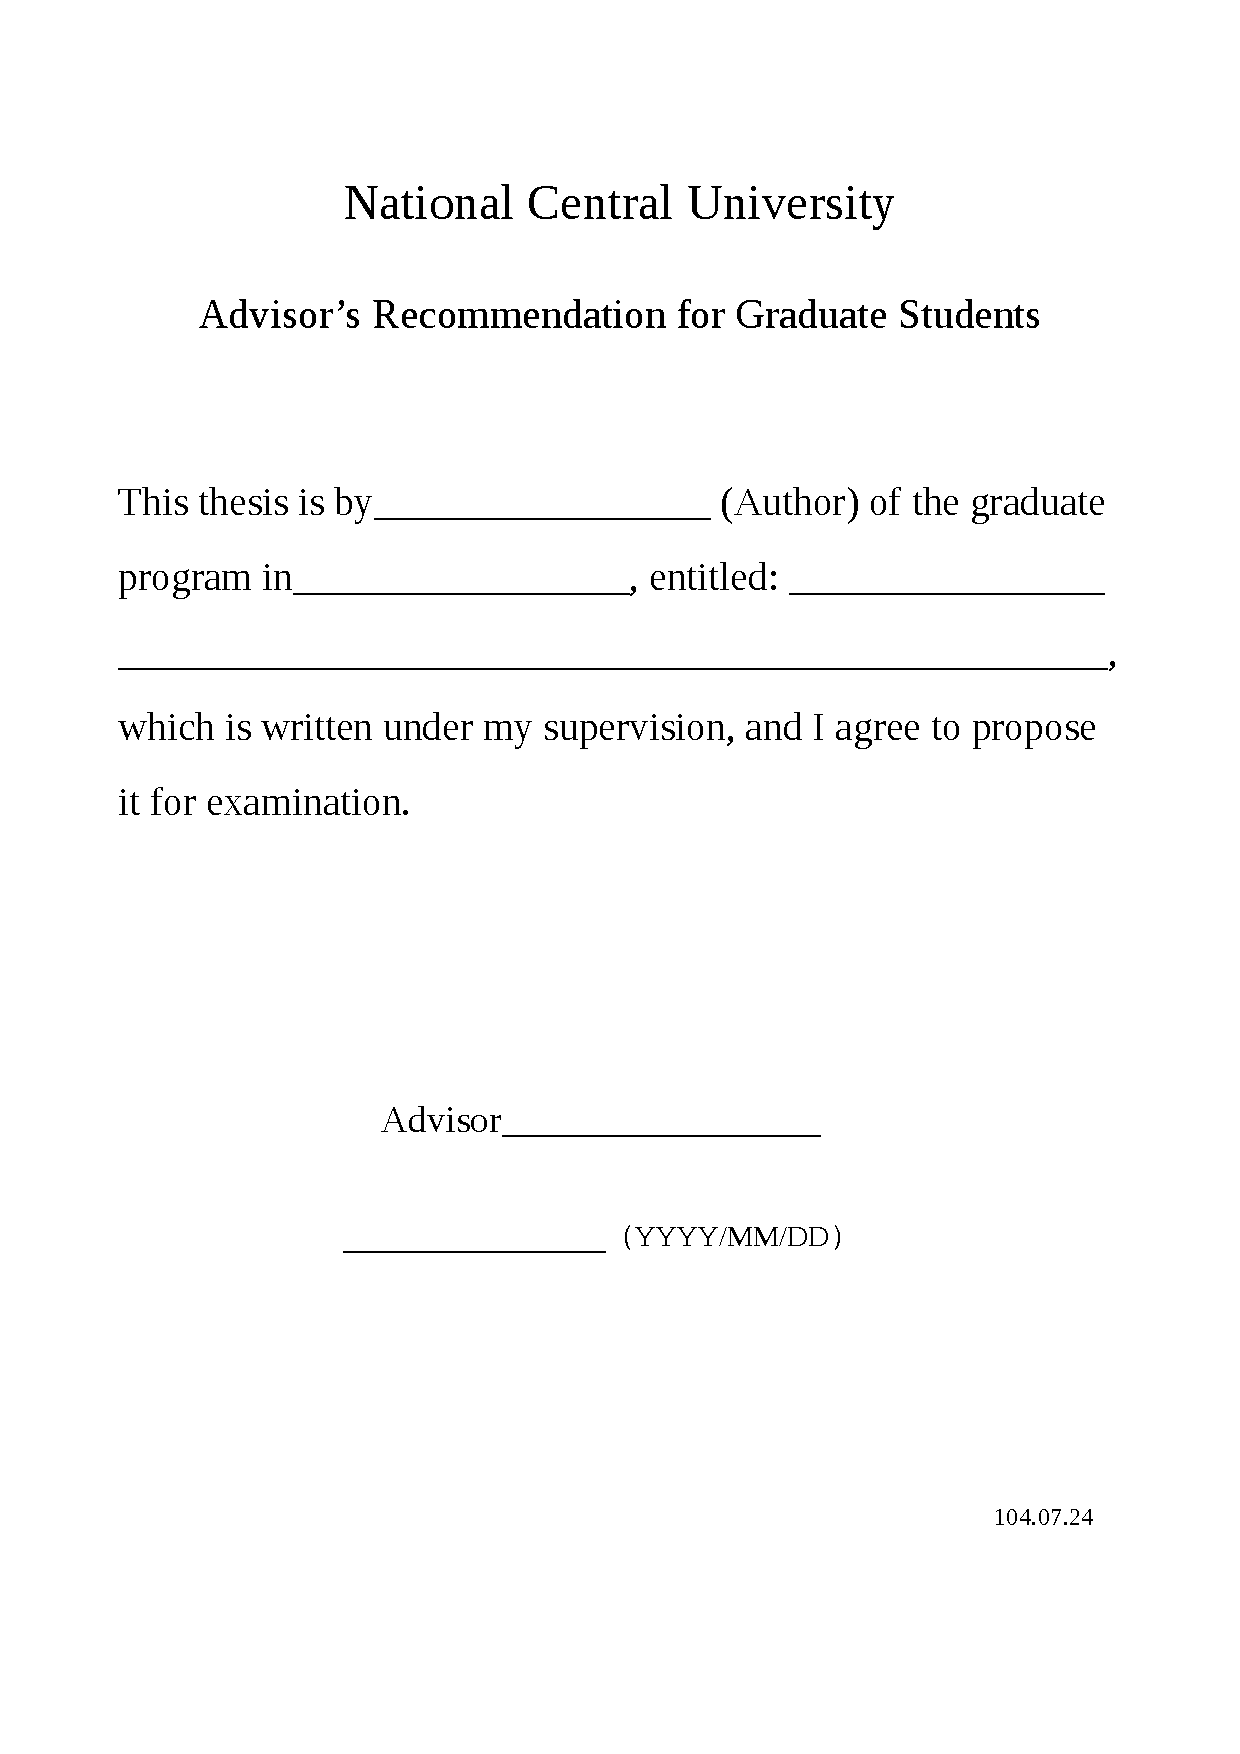
\includepdf[pagecommand={   \placetextbox{50}{159}{\ffs{22}\deptshort}%
                            \placetextbox{118}{159}{\ffs{22}\author}%
                            \placetextbox{105}{144}{\ffs{22}\title}}%
]{letter_recommendation.pdf}}{}

% 口試委員審定書
\IfFileExists{letter_verification.pdf}{
\cleardoublepage\thispagestyle{empty}

\includepdf[pagecommand={   \placetextbox{63}{200.5}{\ffs{22}\deptshort}%
                            \placetextbox{145}{200.5}{\ffs{22}\author}%
                            \placetextbox{100}{170}{\ffs{22}\title}}%
]{letter_verification.pdf}}{}

% ------------------------------
\pagestyle{fancy}
\end{document}
\end{document}
